% !TEX encoding = UTF-8 Unicode

\documentclass[a4paper,12pt]{article}
\usepackage[swedish]{babel}
\usepackage[utf8]{inputenc}
\usepackage{graphicx}
\usepackage{epstopdf}
\usepackage{gensymb}
%% Definitioner för LIPS-dokument

\usepackage[swedish]{babel}
\usepackage[utf8]{inputenc}
\usepackage[T1]{fontenc}
\usepackage{times}
\usepackage{ifthen}

\usepackage[margin=25mm]{geometry}

\usepackage{fancyhdr}
\pagestyle{fancy}
\lhead{}
\chead{\textbf{\LIPSprojekttitel}}
\rhead{\textbf{\textsl{LiTH}}\\\textbf{\LIPSdatum}}
\lfoot{\textbf{\LIPSkursnamn}\\\textbf{\LIPSdokumentansvarig}}
\cfoot{\textbf{\LIPSprojektgrupp}\\\textbf{\LIPSgruppepost}}
\rfoot{\textbf{\textsc{Lip}s}\\\textbf{Sida~\thepage}}

\setlength{\parindent}{0pt}
\setlength{\parskip}{1ex plus 0.5ex minus 0.2ex}


\newcommand{\twodigit}[1]{\ifthenelse{#1<10}{0}{}{#1}}
\newcommand{\dagensdatum}{\number\year-\twodigit{\number\month}-\twodigit{\number\day}}

%% ------------------------------------------
% NYBILD
% Skapar centrerad bild med caption
%   
% #1: Filens url relativt '/bilder/'
% #2:  Caption
% #3: Label
% #4: Skalning
%% ------------------------------------------
\newcommand{\nyBild}[4] 
{\begin{figure}[H]
  \centering
 \includegraphics[angle=0,scale=#4]{bilder/#1}
  \caption{#2}
  \label{fig:#3}
\end{figure}}



%%  Redefinitions of commands containing @
\makeatletter
\makeatother

\newcommand{\LIPStitelsida}{%
{\ }\vspace{45mm}
\begin{center}
  \textbf{\Huge \LIPSdokumenttyp}
\end{center}
\begin{center}
  {\Large Redaktör: \LIPSredaktor}
\end{center}
\begin{center}
  {\Large \textbf{Version \LIPSversion}}
\end{center}
\vfill
\begin{center}
  {\large Status}\\[1.5ex]
  \begin{tabular}{|*{3}{p{40mm}|}}
    \hline
    Granskad & \LIPSgranskare & \LIPSgranskatdatum \\
    \hline
    Godkänd & \LIPSgodkannare & \LIPSgodkantdatum \\
    \hline
  \end{tabular}
\end{center}
\newpage
}


\newenvironment{LIPSprojektidentitet}{%
{\ }\vspace{45mm}
\begin{center}
  {\Large PROJEKTIDENTITET}\\[0.5ex]
  {\small
  \LIPSartaltermin, \LIPSprojektgrupp\\
  Linköpings Tekniska Högskola, ISY
  }
\end{center}
\begin{center}
  {\small Gruppdeltagare}\\
%  \begin{tabular}{|p{30mm}|p{40mm}|p{35mm}|p{45mm}|}
  \begin{tabular}{|l|p{45mm}|p{25mm}|l|}
    \hline
    \textbf{Namn} & \textbf{Ansvar} & \textbf{Telefon} & \textbf{E-post} \\
    \hline
}%
{%
    \hline
  \end{tabular}
\end{center}
\begin{center}
  {\small
    \textbf{E-postlista för hela gruppen}: \LIPSgruppepost\\
    \textbf{Hemsida}: \LIPSgrupphemsida\\[1ex]
    \textbf{Kund}: \LIPSkund\\
    \textbf{Kontaktperson hos kund}: \LIPSkundkontakt\\
    \textbf{Kursansvarig}: \LIPSkursansvarig\\
    \textbf{Handledare}: \LIPShandledare\\
  }
\end{center}
\newpage
}
\newcommand{\LIPSgruppmedlem}[4]{\hline {#1} & {#2} & {#3} & {#4} \\}



\newenvironment{LIPSdokumenthistorik}{%
\begin{center}
  Dokumenthistorik\\[1ex]
  \begin{small}
    \begin{tabular}{|l|l|p{60mm}|l|l|}
      \hline
      \textbf{Version} & \textbf{Datum} & \textbf{Utförda förändringar} & \textbf{Utförda av} & \textbf{Granskad} \\
      }%
    {%
      \hline
    \end{tabular}
  \end{small}
\end{center}
}
\newcommand{\LIPSversionsinfo}[5]{\hline {#1} & {#2} & {#3} & {#4} & {#5} \\}

\newcounter{LIPSkravnummer}
\newcounter{LIPSunderkravnummer}[LIPSkravnummer]
\newenvironment{LIPSkravlista}{%
  \begin{tabular}{|p{25mm}|p{25mm}|p{85mm}|p{5mm}|}
    }%
  {%
    \hline
  \end{tabular}
}
\newcommand{\LIPSkrav}[3]{\hline\stepcounter{LIPSkravnummer}\textbf{Krav nr \arabic{LIPSkravnummer}} & \textbf{{#1}} & {#2} & \textbf{{#3}} \\}
\newcommand{\LIPSunderkrav}[3]{\hline\stepcounter{LIPSunderkravnummer}\textbf{Krav nr \arabic{LIPSkravnummer}\Alph{LIPSunderkravnummer}} & \textbf{{#1}} & {#2} & \textbf{{#3}} \\}





%%% Local Variables: 
%%% mode: latex
%%% TeX-master: "kravspec_mall"
%%% End: 



\newcommand{\LIPSartaltermin}{2012/VT}
\newcommand{\LIPSkursnamn}{TSEA27}

\newcommand{\LIPSprojekttitel}{Komborobot}

\newcommand{\LIPSprojektgrupp}{Grupp 17}
\newcommand{\LIPSgruppepost}{komborobot@googlegroups.com}
\newcommand{\LIPSgrupphemsida}{finns ej}

\newcommand{\LIPSdokumentansvarig}{Mattias Jansson}
\newcommand{\LIPSkund}{ISY, Linköpings universitet, 581\ 83 Linköping}
\newcommand{\LIPSkundkontakt}{Tomas Svensson, 013-281368, tomass@isy.liu.se}
\newcommand{\LIPSkursansvarig}{Tomas Svensson, 013-281368, tomass@isy.liu.se}
\newcommand{\LIPShandledare}{}


\newcommand{\LIPSdokumenttyp}{Kravspecifikation}
\newcommand{\LIPSredaktor}{Simon Larsson}
\newcommand{\LIPSversion}{1.1}
\newcommand{\LIPSdatum}{\dagensdatum}

% Förslag till versionshantering:
% döp helt enkelt om filen till [dokument]_vX.Y.tex vid varje revision


\newcommand{\LIPSgranskare}{}
\newcommand{\LIPSgranskatdatum}{}
\newcommand{\LIPSgodkannare}{}
\newcommand{\LIPSgodkantdatum}{}

\begin{document}

\LIPStitelsida

%% Argument till \LIPSgruppmedlem: namn, roll i gruppen, telefonnummer, epost
\begin{LIPSprojektidentitet}
  \LIPSgruppmedlem{Simon Larsson}{Projektledare (PL)}{070-7311646}{simla804@student.liu.se}
  \LIPSgruppmedlem{\LIPSdokumentansvarig}{Dokumentansvarig (DOK)}{073-6837074}{matja307@student.liu.se}
  \LIPSgruppmedlem{Gustav Svensk}{Reglersystem (REG)}{073-6208776}{gussv666@student.liu.se}
  \LIPSgruppmedlem{Johan Jönsson}{Mjukvara (KA)}{073-8305758}{johjo939@student.liu.se}
  \LIPSgruppmedlem{Tobias Andersson}{Hårdvara (HV)}{073-7201098}{toban963@student.liu.se}
  \LIPSgruppmedlem{Markus Falck}{Leveransansvarig (LV)}{076-3457552}{marlo265@student.liu.se}
  \LIPSgruppmedlem{Simon Wallin}{Testansvarig (GM)}{076-2300665}{simwa252@student.liu.se}
\end{LIPSprojektidentitet}

\tableofcontents{}
\newpage

%% Argument till \LIPSversionsinfo: versionsnummer, datum, ändringar, utfört av, granskat av
\addcontentsline{toc}{section}{Dokumenthistorik}
\begin{LIPSdokumenthistorik}
\LIPSversionsinfo{0.1}{2012-01-26}{Första utkast.}{matja307}{}
\LIPSversionsinfo{0.2}{2012-01-30}{Andra utkast.}{matja307}{johjo939}
\LIPSversionsinfo{1.0}{2012-01-31}{Första versionen}{gussv666}{johjo939}
\LIPSversionsinfo{1.1}{2012-05-07}{Ändrat så att all kommunikation mellan robotens enheter sker via komunikationsenheten. Krav 9 ändrat och krav 28 samt 29 sammanslagna. Vissa redaktionella ändringar för att förtydliga}{simwa252}{simla804}

\end{LIPSdokumenthistorik}
\newpage

\section{Inledning}
I detta dokument formuleras samtliga krav som Komboroboten som beställare Tomas Svensson beställt av Grupp 17 ska uppfylla. 
Komboroboten ska vara enhetsuppbyggd och bestå av en kommunikationsenhet, en styrenhet och en sensorenhet.
Den ska ha ett läge för manuell styrning via blåtand samt ett läge för 
att autonomt kunna följa en bana bestående av antingen en linje längs underlaget, en labyrint med väggar längs sidorna, eller en kombination av de två föregående enligt banspecifikation (A.1).


I samband med leverans ska Komboroboten delta i en tävling där konstruktionen utvärderas.

Prioritetsnivåer enligt \ref{DEF}.

%\includegraphics[scale=.7]{Tsea29.pdf}


% Argument till \LIPSkrav och \LIPSunderkrav: förändring, kravtext, prioritet
\begin{LIPSkravlista}
  \LIPSkrav{Original}{Roboten ska vara enhetsuppbyggd}{1}
\end{LIPSkravlista}

\subsection{Parter}
Beställare: Tomas Svensson \\
Leverantör: Grupp 17

\subsection{Mål}
I samband med leveransen ska roboten klara av att under tävling helt autonomt navigera
en bana som är uppbyggd enligt bestämmelserna i den bifogade banspecifikationen (\ref{app:bana}). 
 Tävlingen avgörs på tid, den robot som tar sig runt banan på kortast tid vinner.

\subsection{Användning}
Roboten ska ha ett autonomt läge och ett fjärrstyrningsläge.
Man ska kunna växla mellan de två lägena med en brytarknapp på roboten.

\subsubsection{Autonomt läge}
I autonomt läge ska roboten kunna startas med en knapp. Den ska då autonomt kunna följa en bana byggd enligt överenskommen banspecifikation (A.1).

\subsubsection{Fjärrstyrningsläge}
I fjärrstyrningsläge ska roboten kunna styras manuellt med en PC via medföljande mjukvara.
Följande kommandon ska finnas: kör framåt, kör bakåt, högersväng, vänstersväng, vänsterrotation, högerrotation och stopp. 
I autonomt läge ska roboten kunna startas med en knapp. Den ska då autonomt kunna följa en bana byggd enligt överenskommen banspecifikation. 


\subsection{Bakgrundsinformation}
Beställaren har givit leverantören i uppdrag att konstruera en robot som uppfyller vissa krav.
Ytterligare en leverantör ska konstruera en liknande robot,
och i samband med tävlingen som hålls under vecka 20 utses vilken av robotarna som bäst tillgodoser beställarens krav.

\subsection{Definitioner} \label{DEF}
\begin{itemize}
\item Prioritetsnivå 1 - Dessa krav ska uppfyllas
\item Prioritetsnivå 2 - Dessa krav ska uppfyllas i mån av tid
\item Prioritetsnivå 3 - Dessa krav ska uppfyllas i mån av tid och efter alla krav med prioritet 2 uppfyllts
\end{itemize}

\section{översikt av systemet}

\subsection{Grov beskrivning av produkten}
Produkten är en komborobot som ska kunna styras trådlöst via blåtand samt autonomt följa linjer och navigera simpla labyrinter.

\begin{figure}[h!]
	\caption{översikt}
	\begin{center}
		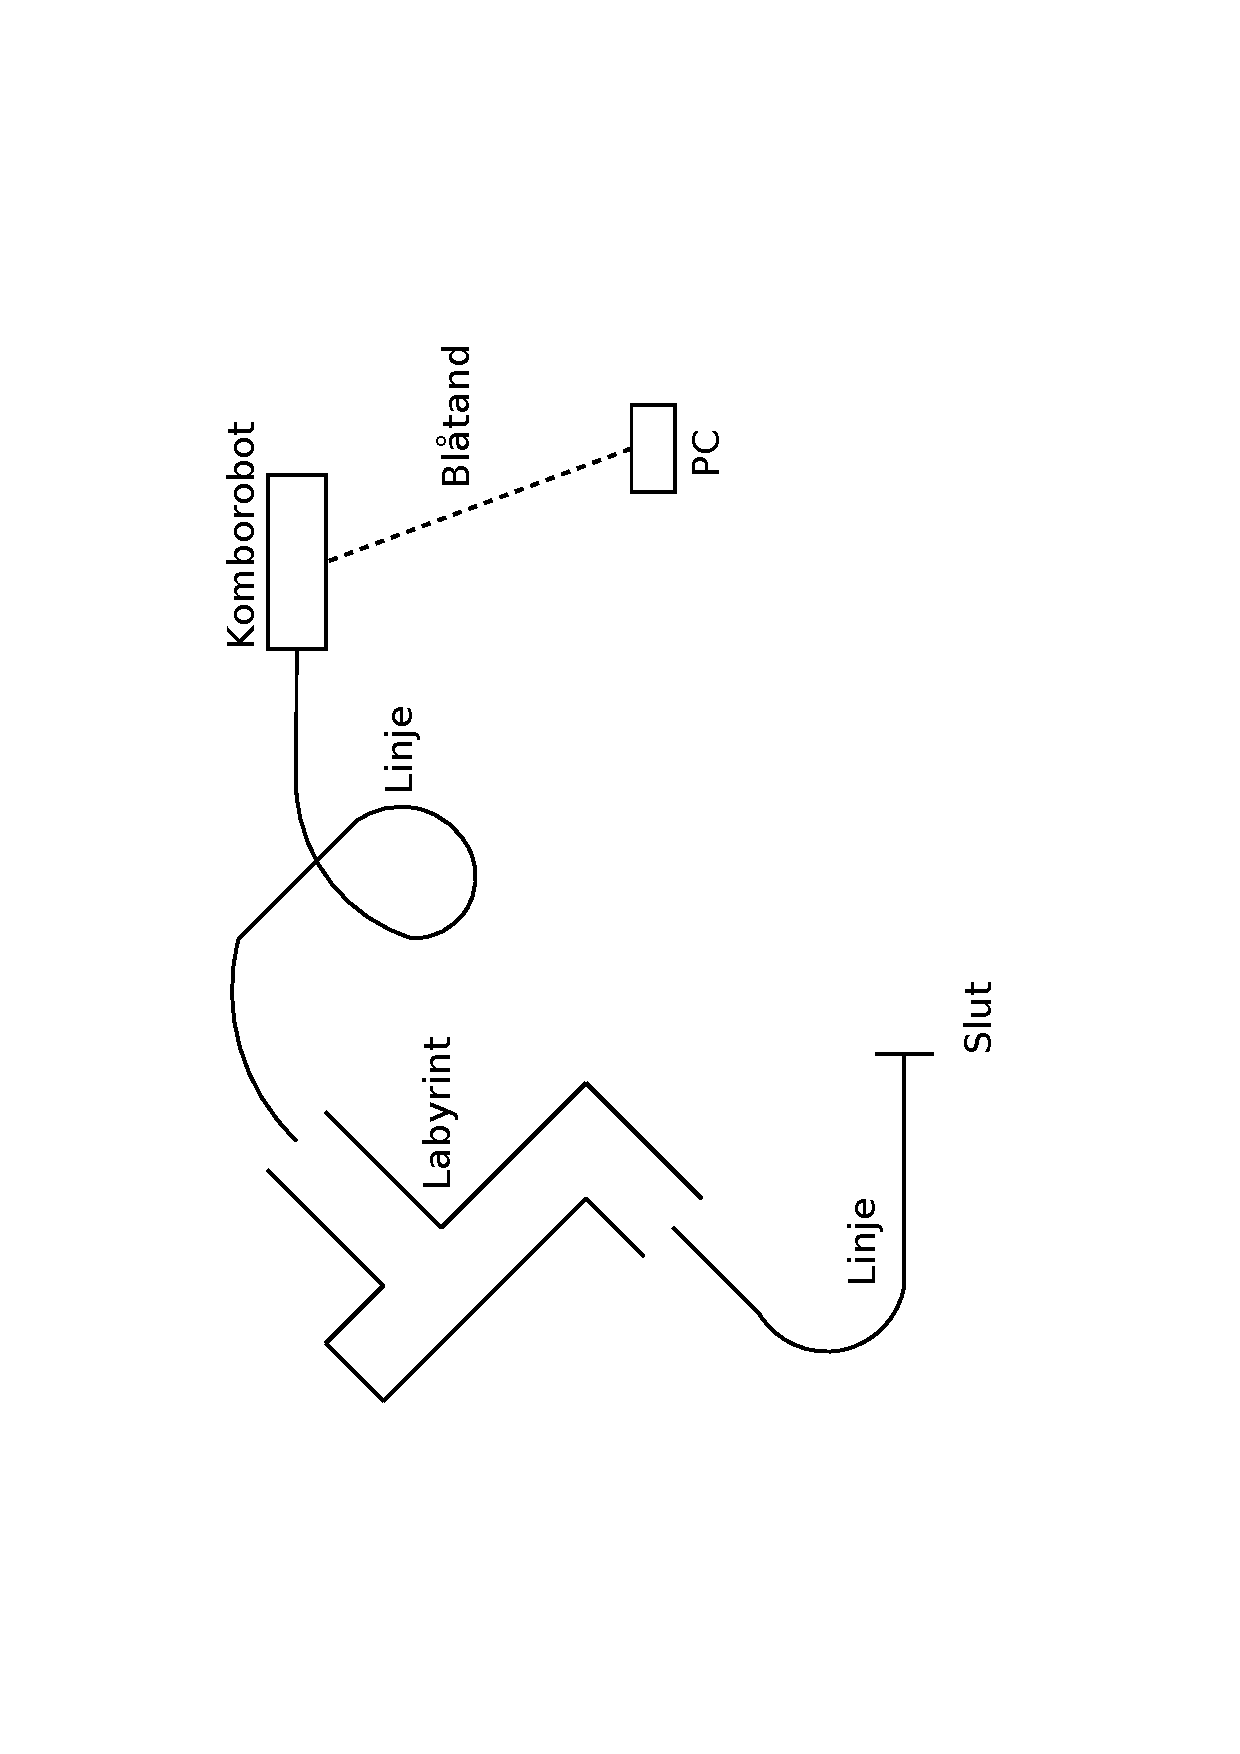
\includegraphics[scale=0.5,angle=270]{Oversikt.pdf}
	\end{center}
\end{figure}

\subsection{Produktkomponenter}
De komponenter som ska ingå i den slutgiltiga produkten är
komboroboten med tillhörande teknisk dokumentation, användarmanual och programvara.

\subsection{Beroenden till andra system}
När roboten är i fjärrstyrningsläge så ska den styras från en PC 
med blåtandsanslutning och den mjukvara som levereras tillsammans med roboten.

\subsection{Ingående delsystem}
De delsystem som ska ingå är en styrenhet som sköter motorer och styrning,
en sensorenhet som sköter tolkning och insamling av data,
en kommunikationsenhet som sköter kommunikation mellan externa och interna enheter samt mjukvara 
som ska installeras på en extern PC som kan visa information om 
styrning och som också kan styra roboten när den är i fjärrstyrningsläge.

\begin{figure}[h!]
	\caption{Delsystem}
	\begin{center}
		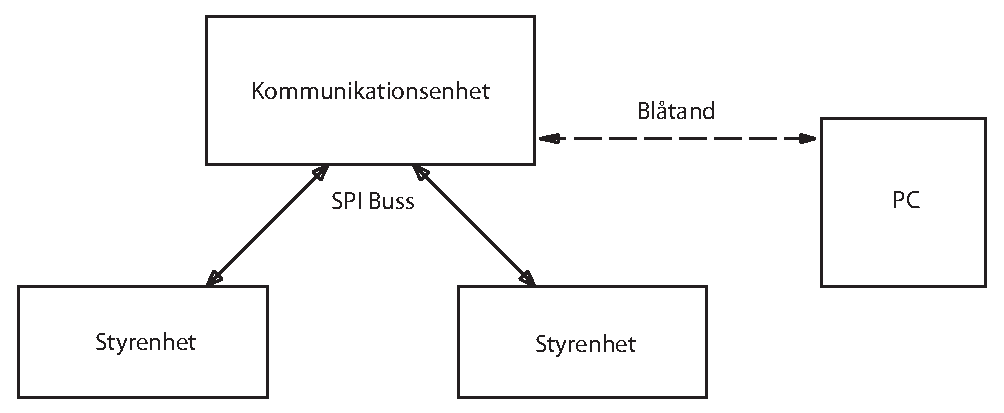
\includegraphics[scale=0.8,angle=0]{delsystem2.pdf}
	\end{center}
\end{figure}

\subsection{Avgränsningar}
Roboten behöver bara klara de banor som beskrivs i banreglerna (\ref{app:bana}).

\subsection{Generella krav på hela systemet}
Systemet i sin helhet ska uppfylla följande krav.

\begin{LIPSkravlista}
  \LIPSkrav{Original}{Roboten ska kunna styras med blåtand}{1} 
  \LIPSkrav{Original}{Roboten ska kunna köra autonomt genom en bana enligt (\ref{app:bana})}{1}
  \LIPSkrav{Original}{Val mellan fjärrstyrnings- och autonomt läge ska styras med en brytare}{1}
  \LIPSkrav{Original}{Roboten ska ha en knapp som startar den i tävlingen}{1}
  \LIPSkrav{Original}{Roboten ska bestå av minst tre enheter, styrenhet, kommunikationsenhet och sensorenhet}{1}
\end{LIPSkravlista}


\section{Styrenhet}
\subsection{Inledande beskrivning}
Styrenheten ska kontrollera alla motorer och servo utifrån data ifrån sensorenheten och kommunikationsenheten.

\subsection{Gränssnitt}
\begin{LIPSkravlista}
  \LIPSkrav{Original}{Felmeddelanden ska skickas till kommunikationsenheten}{1} 
  \LIPSkrav{Original}{Information om robotens nuvarande aktivitet, t ex svänger vänster, ska skickas till kommunikationsenheten när roboten är i autonomt läge}{1} 
  \LIPSkrav{Ändrat 2012-05-07}{Styrdata ska kunna tas emot från kommunkationsenheten och från sensorenheten via kommunikationsenhetn}{1} 
\end{LIPSkravlista}

\subsection{Designkrav}
Styrenheten ska designas så att den kan bytas ut mot en annan styrenhet med t ex en annan styralgoritm.

\begin{LIPSkravlista}
	\LIPSkrav{Original}{Styrenheten ska innehålla minst en processor}{1}
	\LIPSkrav{Original}{Styrenheten ska kunna bytas ut}{1}
\end{LIPSkravlista}

\subsection{Funktionella krav}
\begin{LIPSkravlista}
	\LIPSkrav{Original}{Roboten ska följa en linje eller en korridor specificerad enligt banspecifikation (\ref{app:bana}) utan att slingra sig fram}{1}
  \LIPSkrav{Original}{Roboten ska kunna utföra följande kommandon: fram, fram vänster, fram höger, back, rotera vänster, rotera höger och stopp}{1}
\end{LIPSkravlista}

\section{Kommunikationsenhet}
\subsection{Inledande beskrivning}
Komboroboten ska kunna kommunicera med en dator via blåtand.
Kommunikationsenheten ansvarar för att skicka data från komborobotens 
sensorenhet och styrenhet till en datorn, via blåtand.
I fjärrstyrningsläge skall även kommunikationsneheten ta emot 
instruktioner och information från datorn, via blåtand.
Dessa instruktioner och data kan sedan användas för att styra komboroboten.


\begin{LIPSkravlista}
  \LIPSkrav{Original}{Kommunikationsenheten ska skicka data, exempelvis felmeddelanden till datorn via blåtand}{1}
  \LIPSkrav{Original}{Kommunikationsenheten ska ta emot data, exempelvis instruktioner till styrenheten via blåtand}{1}
  \LIPSkrav{Original}{Kommunikationsenheten ska skicka data från datorn till lämplig enhet, exempelvis navigationsinstruktioner skickas till styrenheten}{1}
\end{LIPSkravlista}

\subsection{Externa interface}
Kommuniaktionsenheten ska kommunicera med övriga enheter på roboten samt datorn och förmedla information mellan dessa.


\begin{LIPSkravlista}
  \LIPSkrav{Original}{Kommunikationsenheten ska ta emot data från sensorenheten och förmedla den till datorn, via blåtand}{1}
  \LIPSkrav{Original}{Kommunikationsenheten ska ta emot data från styrenheten och skicka denna vidare till datorn, via blåtand}{1}
\end{LIPSkravlista}

\subsection{Designkrav}
Kommunikationsenheten ska designas på så sätt att den enkelt kan bytas ut mot en annan kommunikationsenhet,
t.ex. för kommunikation via annan standard än blåtand


\begin{LIPSkravlista}
  \LIPSkrav{Original}{Kommunikationsenheten ska innehålla minst en processor}{1}
\end{LIPSkravlista}

\subsection{Funktionella krav}
Det ska vara möjligt att helt kunna styra komboroboten via blåtand då roboten befinner sig i fjärrstyrt läge.


\begin{LIPSkravlista}
  \LIPSkrav{Original}{Roboten ska kunna fjärrstyras via blåtand}{1}
  \LIPSkrav{Original}{Kommunikationsenheten ska fysiskt kunna visa blåtandsaktiviteten}{2}
\end{LIPSkravlista}

\section{Sensorenhet}
\subsection{Inledande beskrivning}
Sensorenheten hämtar data från avståndssensorerna samt linjesensorerna 
och skickar dessa vidare till kommunikationsenheten som sedan förmedlar det till styrenheten. 
Sensorenheten skall även kunna kalibrera linjeföljarsensorn om det är önskvärt.


\begin{LIPSkravlista}
  \LIPSkrav{Original}{Sensordata för avstånd till väggarna på sidan om roboten skall samlas in}{1}
  \LIPSkrav{Original}{sensorenheten ska med sensordata från linjeföljarsensorerna kunna märka skillnader mellan golv och svart tejp på marken}{1}
  \LIPSkrav{Original}{Sensorenhetens linjeföljarsensorer ska kunna kalibreras}{1}
  \LIPSkrav{Original}{Sensorenhetens linjeföljarsensorer ska kunna kalibreras trådlöst via bluetooth}{2}
\end{LIPSkravlista}

\subsection{Externa interface}
\begin{LIPSkravlista}
  \LIPSkrav{Original}{Sensorenheten ska kunna visa avstånd till väggar på en display}{2}
\end{LIPSkravlista}

\subsection{Designkrav}
Sensorenheten ska kommunicera med kommunikationsenheten samt 
styrenheten och förmedla vidare sensordata.
Enheten ska vara designad så att den är utbytbar med en likvärdig enhet. Enheten ska innehålla minst en processor.


\begin{LIPSkravlista}
  \LIPSkrav{Original}{Sensorenheten ska innehålla minst en processor}{1}
  \LIPSkrav{Ändrat 2012-05-07}{Sensordata ska kontinuerligt skickas till kommunikationsenheten och därifrån vidare till styrenheten}{1}
  \LIPSkrav{Original}{Sensorenheten ska vara utbytbar}{1}
\end{LIPSkravlista}

\subsection{Funktionella krav}
Linjeföljarsensor skall i labyrintläge läsa av markeringar på marken som sedan tolkas av styrenheten.


\begin{LIPSkravlista}
	\LIPSkrav{Original}{Sensorenheten ska kunna läsa av markeringar på marken (se \ref{app:bana} för tydligare beskrivning av markeringar)}{1}
\end{LIPSkravlista} 

\subsection{Användargränssnitt}
\begin{LIPSkravlista}
  \LIPSkrav{Original}{All kommunikation med sensorenheten sker via kommunikationsenheten}{1}
\end{LIPSkravlista}


\section{Datormjukvara}
\subsection{Inledande beskrivning}
För att styra roboten krävs datormjukvara som kan låta användaren skicka kommandon från en dator till robotens kommunikationsenhet. 


\begin{LIPSkravlista}
  \LIPSkrav{Original}{Information om robotens styrbeslut skall kontinuerligt visas på en datorskärm}{1}
  \LIPSkrav{Original}{Förståelig information från sensorenheten skall kontinuerligt visas på en datorskärm}{1}
  \LIPSkrav{Original}{Avståndet till väggarna skall redovisas i cm på en datorskärm}{2}
\end{LIPSkravlista}

\subsection{Designkrav}
\begin{LIPSkravlista}
  \LIPSkrav{Original}{Mjukvaran ska designas på så sätt att man enkelt kan anpassa den ifall någon av robotens enheter byts ut}{1}
\end{LIPSkravlista}

\subsection{Funktionella krav}
Datormjukvaran ger användaren möjlighet att granska information från roboten på en dator.
Användaren ska även kunna styra roboten via mjukvaran då roboten befinner sig i fjärrstyrt läge.


\begin{LIPSkravlista}
  \LIPSkrav{Original}{Datormjukvaran ska ge möjlighet att styra roboten då den befinner sig i fjärrstyrt läge}{1}
  \LIPSkrav{Original}{Datormjukvaran ska innehålla ett grafiskt användargränssnitt för att styra roboten i fjärrstyrt läge}{2}
  \LIPSkrav{Original}{Datormjukvaran ska visa information från robotens olika enheter}{1}
  \LIPSkrav{Original}{Datormjukvaran ska via ett grafiskt användargränssnitt visa information från robotens olika enheter}{2}
\end{LIPSkravlista}


\section{Prestandakrav}
Roboten ska klara av att ta sig igenom banor som uppfyller banspecifikationen i tävlingsreglerna.
Roboten ska dessutom följa reglerna som är uppsatta i regeldokumentet när den utför sin uppgift.
Vilken nivå av bana som används till tävlingen ska bestämmas innan tävlingen.
Ett mål är även att minimera tiden det tar för roboten att ta sig genom banan.


\begin{LIPSkravlista}
	\LIPSkrav{Original}{Roboten ska ta sig igenom en bana av nivå 1 som definieras i banspecifikationen (\ref{app:bana})}{1}
        \LIPSkrav{Original}{Roboten ska ta sig igenom en bana av nivå 2 som definieras i banspecifikationen (\ref{app:bana})}{2}
	\LIPSkrav{Original}{Roboten ska ta sig igenom en bana av nivå 3 som definieras i banspecifikationen (\ref{app:bana})}{3}
\end{LIPSkravlista}



\section{Krav på vidareutveckling}
\begin{LIPSkravlista}
  \LIPSkrav{Original}{Samtliga av de olika enheterna på roboten ska ha väl specificerade gränssnitt}{1}
  \LIPSkrav{Original}{Det ska på ett enkelt vis vara möjligt att byta ut enskilda enheterna på roboten}{1}
\end{LIPSkravlista}


\section{Ekonomi}
Efter att projektet har passerat BP2 ska  totalt 980 timmar (140 timmar per projektmedlem) brukas.
\\
\begin{LIPSkravlista}
  \LIPSkrav{Original}{Totalt 980 timmar skall används i projektet efter att projektplanen godkänts}{1}
\end{LIPSkravlista}


\section{Leveranskrav och delleveranser}
Dessa krav specificerar alla de leveranser som ska ske under projektets gång,
och när dessa senast ska vara handledaren och beställaren tillhanda.
Alla leveranser ska senast vara levererade vid 16:00 under det angivna datumet.
Under vecka 20 så ska en slutleverans ske i form av en muntlig presentation, samt en demonstation av roboten.


\begin{LIPSleveranslista}	
	\LIPSleverans{Original}{Kravspecifikation}{2/2-2012}{1}
	\LIPSleverans{Original}{Första version av projektplan, tidplan och systemskiss}{15/2-2012}{1}
	\LIPSleverans{Original}{Slutgiltig version av projektplan, tidplan och systemskiss}{15/2-2012}{1}
	\LIPSleverans{Original}{Första version av designspecifikation}{12/3-2012}{1}
	\LIPSleverans{Original}{Slutgiltig version av designspecifikation}{16/3-2012}{1}
	\LIPSleverans{Original}{Teknisk Dokumentation och användaranvisning}{3 arbetsdagar före redovisningen v20}{1}
	\LIPSleverans{Original}{Efterstudie}{1/6-2012}{1}
	\LIPSleverans{Original}{Tidrapporter}{12/3, 19/3, 26/3, 2/4, 16/4, 23/4, 30/4, 7/5, 14/5, 21/5}{1}
	\LIPSleverans{Original}{Statusrapport}{Vid begäran}{1}
	\LIPSleverans{Original}{Slutleverans innehållande en muntlig presentation på 15-20 minuter samt en demonstation}{Vecka 20}{1}
	\LIPSleverans{Original}{Presentationen ska innehålla grafisk information som presenteras med en projektor}{}{1}
\end{LIPSleveranslista}

\section{Dokumentation}
Dokumentation för projektet innebär följande dokument: 
\begin{list}{*}{}
\item Teknisk dokumentation: Beskriver systemet och dess olika delar
\item Användarmanual: Beskriver på ett änklare sätt hur produkten används
\end{list} 

\begin{LIPSkravlista}	
	\LIPSkrav{Original}{Dokumentation enligt ovan ska finnas vid leverans.}{1}
	\LIPSkrav{Original}{Dokumentationen ska vara tydligt formulerad, samt samt ha en enhetlig layout.}{1}
	\LIPSkrav{Original}{Dokumentationen ska fälja LIPS-standard.}{1}
	\LIPSkrav{Original}{Dokumentation ska skrivas på svenska}{1}
\end{LIPSkravlista}

%\begin{LIPSkravlista}
%\LIPSkrav{Original}{Dokumenten ska ha enhetligt utseende och utgå från LIPS-mallar}{1}
%\LIPSkrav{Original}{Dokument ska märkas med versionsnummer}{1}
%\LIPSkrav{Original}{Möten ska protokollföras enligt LIPS-mallen för mötesprotokoll}{1}
%\LIPSkrav{Original}{Mötesprotokoll ska justeras av två utsedda justeringspersoner}{1}
%\LIPSkrav{Original}{Dokumentation ska skrivas på svenska}{1}
%\end{LIPSkravlista}


\newpage
\appendix
\section{Bilagor} \label{app:rules}
%Version 1.1
%
%2 - 4 Lag
%
%Roboten ska operera autonomt och måste bära med sig den dator som utför
%beräkningarna som krävs för att den ska utföra sin kartläggning.  Detta innebär
%att roboten inte får fjärrstyras från en laptop som utför beräkningarna som
%krävs för att roboten ska navigera etc.  Man får inte tejpa fast en laptop på
%roboten.

%\subsection{Regler}

%En robot per lag.  Roboten ska själv avgöra när kartläggningen är klar och
%signalera det.  Kartan ska under uppritning visas på en skärm eller projektor
%och vara komplett när roboten anser sig klar.  Robotarna kör i tur och ordning
%och börjar i samma ruta, dock inte tvunget vriden åt samma håll.  Robotarna ska
%starta kartläggningen genom att någon trycker på en knapp på roboten.  Den
%robot som snabbast signalerar att den är klar med kartritningen och vars karta
%överrensstämmer med verkligheten får 4 poäng, 2:an får 3 poäng, 3:an får 2
%poäng och fyran får 1 poäng.  Man kör två omgångar och om man i slutet har n
%(n: heltal) par med samma resultat får de spela om sin placering i en 4:de
%omgång.  Ola väljer startpositioner. Laget väljer var på rutan roboten ska
%starta. Ingen del av roboen får vara utanför den designerade rutan vid start.
%Körtiden mäts från det att knappen är tryckt i sekunder tills roboten
%signalerat klar och man kan se en karta på skärmen.
%
%Man får inte ge roboten en hårdkodad verision av banan att arbeta utifrån.
%Roboten ska söka sig fram till kartan inte bara verifiera en existerande
%version.
%
%Om roboten signalerar klar i förtid (innan hela kartan syns på persondatorn)
%läggs 10 sekunder till på dess arbetstid. Dessutom kommer tiden mellan KLAR
%signalen och då hela kartan visas på persondatorn att läggas till robotens tid
%den omgången.  Om kartan är ofullständig 4 minuter efter KLAR signal eller då
%gruppen ger upp får roboten i den omgången 0 poäng.  Om två eller fler robotar
%klarar uppgiften på samma tid så delar de på placeringen och får samma poäng.
%Roboten på platsen efter de två med lika tid får då poängen som den skulle fått
%om den två hade olika bättre tider.  Huruvida tiderna är optimala bör
%förhandlas.

%Vid oklarheter är det Ola Dahl som bedömmer utgången av en omgång eller en
%annan person utsedd av Ola. Ola har också tillåtelse att tilldela/dra ifrån
%sekunder på en omgång.


\subsection{Banspecifikation} \label{app:bana}

%Ska vara uppförd av Ola Dahl eller ersättare tillsatt av Ola Dahl.  Max 8 x 8 rutor
%stor. Varje ruta är 80cm x 80cm. Max 6.4 x 6.4 m. (projektdirektivet anger 6x6m
%vilket är omöjligt) Vara tät, dvs inga hål i yttre väggen får finnas.  Inte ha
%"tunna" väggar. Varje vägg har alltså en otillgänglig ruta bakom sig.  Ha
%väggar beståendes av 80cm långa vita pappskivor som skär varandra i 90 graders
%vinklar.  Maximalt ha en "köksö", "köksön" kan ha godtycklig storlek. "Köksön"
%ska vara placerad passade till det rutnät (grid) man kan bygga upp av
%ytterväggen. "Köksön" består av rutor på samma sätt som övriga banan.

Banan består av två huvuddelar: Linjedelar och labyrintdelar, där linjerna fungerar som transportsträcka till, från eller mellan en eller flera labyrinter. Linjen tar vid i mitten av labyrintgången 5 cm in i labyrinten där den slutar eller börjar. Labyrintens beståndsdelar varierar utifrån vilken prioritetsnivå som är uppfylld. Tävlingsdeltagarna kommer innan tävlingen överens om vilken av nivåerna som ska användas.
\\
\\
Linjedelen:
\\
Linjerna i banan skall bestå av en svart tejp på grått underlag. Tejpens bredd ska vara mellan 14-18 mm. I de fall en tjock linje nämns avses en tejplinje med bredd mellan 42-54 mm (tre tejpbredder). Med en smal tejplinje avses en linje med bredd 14-18 mm (en tjepbredd). Tejpbanan kan korsa sig själv i 90\degree korsningar, den kan dock ej dela sig. Svängradien för banan är minst 25 cm. Banan avslutas med en stoppsignal eller övergår till en labyrint. Stoppsignalen inleds med en 30 cm raksträcka som sedan övergår i en tvärgående linje följt av tre parallella smala linjer, 1 tejbredd isär med mitten där den tidigare linjen avslutades, i färdriktningen. Banan kan endast avslutas i linje läge och aldrig i en labyrint.
\\


Labyrintdelen:

\begin{list}{*}{}
\item Nivå 1: Avståndet mellan parallella väggar är 80 cm. 3-vägskorsningar och 4-vägskorsningar kan förekomma, dock med räta vinklar mellan varandra, rätt väg anges av markeringar på golvet. Markeringarna görs med två linjer som går vinkelrätt mellan väggarna. En tjock linje följd av en tunn indikerar höger, en tunn följd av en tjock indikerar vänster och två linjer av samma tjocklek rakt fram. Markeringarna ska vara 50 cm breda och liga 15 cm från vardera sida av labyrinten. En raksträcka på 25 cm ska följa fram till korsningen. 
\item Nivå 2: Som nivå 1 med följande justeringar: Inga markeringar behövs då ena vägen vid en korsning är en återvändsgränd med djup på 80 cm.
\item Nivå 3: Som nivå 1 med följande justeringar: Inga markeringar nödvändiga. Hål 80 cm stora ut ur labyrinten som inte leder någonstans kan förekomma.
\end{list} 

\begin{figure}[h!]
	
	\begin{center}
		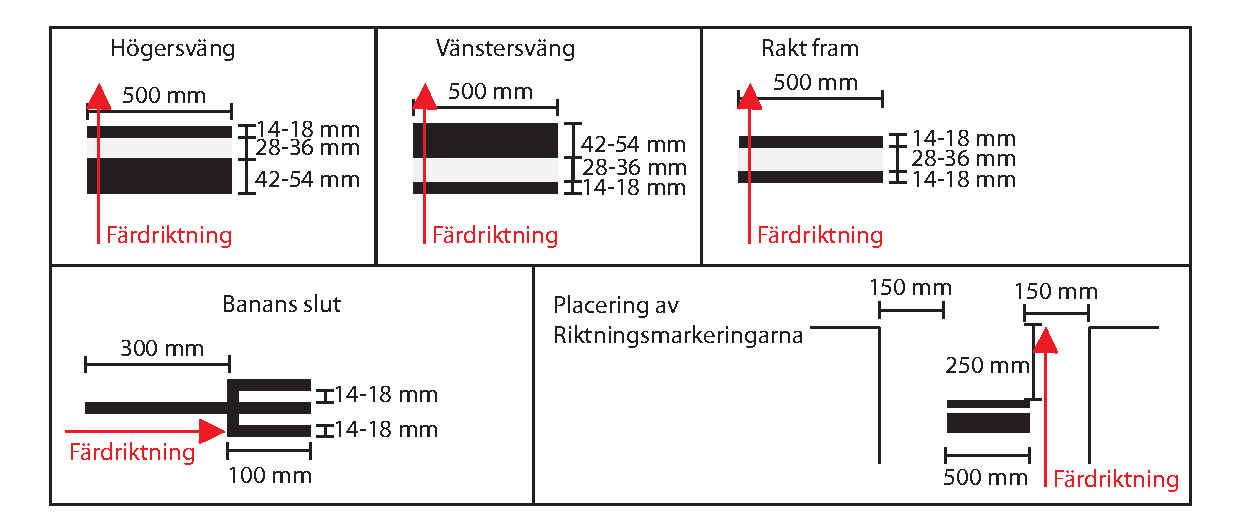
\includegraphics[scale=0.5,angle=0]{Rikningsmarkerinag_stopp.pdf}
	\end{center}
	\caption{Riktnings- och stoppmarkeringar samt placering}
\end{figure}

\newpage


\addcontentsline{toc}{section}{Referenser}
\begin{thebibliography}{99}
\bibitem{lipskompendiet}\textit{Projektmodellen LIPS - } Svensson, Tomas
\\Studentlitteratur, 2011.
\end{thebibliography}


\end{document} 


%%% Local Variables: 
%%% mode: latex
%%% TeX-master: t
%%% End: 
